
\documentclass[paper=a4, fontsize=12pt]{article} % A4 paper and 11pt font size

\usepackage{xepersian}
\usepackage{graphics}
\settextfont{XB Niloofar}
\renewcommand{\baselinestretch}{1.5}
%\usepackage{amsmath}
%\usepackage{mathtools}



\begin{document}

\begin{titlepage}
\begin{center}


\includegraphics[width=3.38cm]{amirkabir.jpg}\\[5pt]
{\Large\bfseries 
دانشگاه صنعتی امیرکبیر
}\\
\linespread{1}
{\Large
(پلی تکنیک تهران)
}\\
{\LARGE
دانشکده مهندسی برق
}\\
 % ----------------------------------------------------------------
 \vspace{1.5cm}

 {\LARGE\bfseries
پروژه درس بینایی ماشین
 }\\
% ----------------------------------------------------------------
 \vspace{1.5cm}
%\settextfont{IranNastaliq}
{\huge\bfseries 
روش دنبال کردن تصویر متناسب با مقدار بزرگنمایی آن برپایه روش جابجایی میانگین
\\
و استفاده از ویژگی های کارآمد
\\}
 % ----------------------------------------------------------------
 \vspace{1.5cm}
 {\Large\bfseries
دانشجو: محمد حسن شماخی 
 }\\

 mh.shammakhi@aut.ac.ir\\[14pt]
  % ----------------------------------------------------------------
 \vspace{1cm}

 {\Large\bfseries
استاد درس: دکتر فائز
 }\\
 % ----------------------------------------------------------------
 \vfill
{
زمستان 94
}		
              
\end{center}
\end{titlepage}






\tableofcontents
\newpage

\section{مقدمه}
ردیابی بی درنگ \footnote{Online}  دارای کاربردهای وسیعی در زمینه نظارت، کمک به رانندگان و رباتیک می‌باشد و نقش بسیار مهمی در کاربردهای شناسایی الگو ایفا می‌کند.
ردیابی به روش جابه‌جایی میانگین اولین بار حدود 10 سال پیش در
~\cite{1Bedfold}
 معرفی‌شد و به دلیل پیچیدگی محاسباتی پایین، موفقیت بسیاری در ردیابی برخط به دست آورد. اما در مواردی که ابعاد جسم به مرور تغییر می‌کند، این روش دچار ضعف می‌شود و بازدهی بالایی ندارد. راه‌حل‌های مختلفی برای غلبه بر این مشکل پیشنهاد شده است. از جمله استفاده از هرم تصویر با مقیاس‌های مختلف و جستجو در تمام تصاویر آن برای پیدا کردن محتمل ترین مکان جسم
\cite{2SVT}
است.
این روش‌ها بار محاسباتی بالایی دارند و استفاده از آن‌ها برای تعیین ابعاد جسم می‌تواند قابلیت انجام ردیابی به‌صورت برخط را از بین ببرد. به همین دلیل روش‌های دیگری مبتنی بر استخراج الگو و ردیابی این الگو مطرح شدند. به این صورت که از پنجره موردنظر برای ردیابی، الگو استخراج‌شده و در مدت ردیابی این الگو با نواحی مختلف تصویر مقایسه می‌شود و مشابه‌ترین الگو به‌عنوان مکان بعدی جسم معرفی می‌شود. یکی از مطرح‌ترین این روش‌ها در
\cite{3Oikonomidis}
 معرفی‌شده است. همچنین در
\cite{4Zhang}
  الگوی ORB \footnote{Oriented FAST and Rotated BRIEF (Binary Robust Independent Elementary Features)} در سال 2011 معرفی شد که به دلیل پربازده بودن می‌تواند جایگزین SIFT \footnote{Scale-Adaptive Feature Transform} شود و همچنین در مسئله ردیابی نیز به‌عنوان الگوی مورد ردیابی، بکار برده شود.
در این مقاله ایده اصلی ترکیب ردیابی به روش جابه‌جایی میانگین، و انطباق الگو می‌باشد. به این صورت که روش اصلی مورد استفاده، استفاده از جابه‌جایی برای پیدا کردن محتمل‌ترین مکان جسم در فریم‌های بعدی و باهمین ابعاد فریم قبل می‌باشد. سپس نقاط متناظری از دو فریم تصویر پیدا می‌شود و با انطباق این نقاط میزان تغییر ابعاد تصویر به دست می‌آید. با این کار هم میزان پیچیدگی محاسباتی کاهش چشمگیری پیدا می‌کند و هم دقت پیدا کردن مقیاس جسم افزایش پیدا می‌کند.
در قسمت اول این گزارش الگوریتم مورد استفاده توسط مقاله برای ردیابی اجسام مورد بررسی قرار می‌گیرد و درباره نقاط ضعف و قوت آن بحث می‌شود. همچنین نتایج شبیه‌سازی روش مورد استفاده مقاله بیان و مورد بررسی قرار می‌گیرد. در بخش دوم پیشنهاد‌هایی برای بهبود عملکرد این روش هم از دقت و هم پیچیدگی محاسباتی بیان می‌شود و نتایج شبیه‌سازی آن مورد بررسی قرار می‌گیرد.
\section{	ردیابی به روش جابه‌جایی و انطباق ویژگی}
ردیابی یک جسم شامل دو مرحله می‌باشد.
\begin{enumerate}
\item مدل‌سازی هدف
\item ردیابی هدف
\end{enumerate}
در مرحله اول جسم موردنظر شناسایی می‌شود و یا توسط کاربر مشخص می‌شود، سپس با استفاده از روشی که از پیش درنظرگرفته‌شده‌است، به مدل‌سازی هدف پرداخته می‌شود. یعنی از جسم مشخص‌شده، مدلی برای انطباق با فریم‌های بعدی به دست می‌آید. این مدل می‌تواند مکان جسم، هیستوگرام رنگ و یا حتی نتیجه اعمال یک توصیف‌گر بافت بر روی آن باشد.
در مرحله دوم از نتیجه مدل‌سازی در مرحله اول استفاده می‌شود و با توجه به مدل ساخته‌شده، الگوریتمی برای پیدا کردن شبیه‌ترین مدل به آن در فریم بعدی پیشنهاد می‌شود. این الگوریتم می‌تواند استفاده از فیلتر کالمن برای پیش‌بینی مکان بعدی جسم، و یا روشی دیگر مانند جابه‌جایی میانگین برای پیدا کردن شبیه‌ترین الگو به الگوی فریم قبلی باشد.
به‌طور مثال در شکل \ref{pic-1} تصویر چهره شخص با استفاده از توصیف‌گر بافت LBP \footnote{Local Binary Pattern} مدل‌سازی شده است و هیستوگرام آن به‌عنوان الگوی مورد ردیابی استخراج‌شده است. سپس در فریم‌های بعدی، این الگو با سایر الگوهایی که از آن فریم استخراج می‌شود مقایسه شده و شبیه‌ترین آن‌ها به‌عنوان مکان بعدی چهره شخص در نظر گرفته می‌شود.
\begin{figure}[h]
\centering
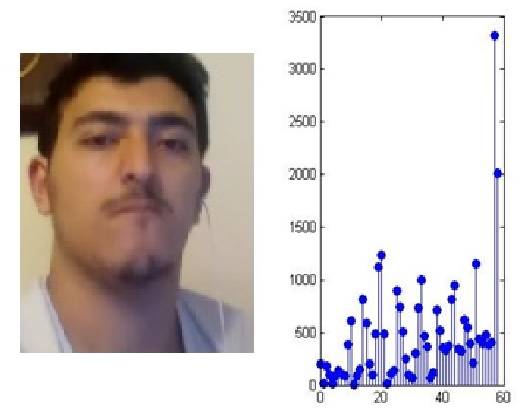
\includegraphics[scale=0.8]{fig1.jpg}
\caption{مدل‌سازی یک تصویر برای ردیابی}
\label{pic-1}
\end{figure}


در این مقاله از روش جابه‌جایی میانگین برای پیدا کردن مکان تقریبی جسم در فریم بعدی استفاده می‌شود. سپس با استفاده از استخراج الگو از نقاطی خاص از تصاویر در فریم‌های قبلی و بعدی، مقدار تغییر ابعاد جسم بین دو فریم مشخص‌شده و مکان جسم به‌طور دقیق پیدا می‌شود. این روند در شکل \ref{pic-2} نشان داده‌شده است.
\begin{figure}[h]
\centering
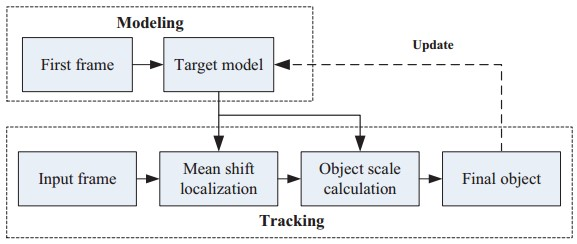
\includegraphics[scale=0.8]{fig2.jpg}
\caption{الگوریتم مورد استفاده مقاله برای استفاده از الگو در ردیابی به روش جابه‌جایی میانگین}
\label{pic-2}
\end{figure}
همان‌طور که در شکل \ref{pic-2} مشاهده می‌شود، ابتدا در فریم اول تصویر، پنجره مورد ردیابی توسط کاربر مشخص می‌شود و از این بخش مورد هدف، الگو استخراج می‌شود. با آمدن فریم‌های بعدی، ابتدا این فریم وارد بخش ردیابی Mean-Shift می‌شود تا مکان تقریبی جسم در این فریم پیدا شود، سپس با استفاده از این مکان تقریبی و مکان جسم در فریم قبلی، ابعاد جسم در فریم جدید محاسبه می‌شود و درنهایت مکان دقیق جسم به دست می‌آید. بعد از پیدا شدن مکان دقیق جسم، به‌منظور در نظر گرفتن تغییرات تدریجی ظاهر جسم مورد ردیابی، از این جسم در فریم کنونی الگو استخراج‌شده و برای به‌روزرسانی الگوی اصلی استفاده می‌شود.
در این بخش از گزارش ابتدا نحوه انجام ردیابی به روش Mean-Shift توضیح داده می‌شود. سپس نحوه محاسبه ابعاد جسم در فریم کنونی بیان می‌شود. در قسمت آخر این بخش نیز، نحوه‌ی به‌روزرسانی الگوی استخراج‌شده از جسم مورد ردیابی تشریح می‌شود.
\subsection{ ردیابی به روش جابه‌جایی میانگین} 
\footnote{Mean-Shift}
روش جابه‌جایی میانگین درواقع روشی تکراری برای پیدا کردن ماکزیمم یک تابع است. با استفاده از این روش می‌توان به‌طور بهینه و با دقت دلخواه،  اکسترمم تابع را تعیین کرد. روش انجام این کار در شکل \ref{pic-3} آورده شده است.
فرض کنید قصد داریم ماکزیمم یک تابع چگالی احتمال را پیدا کنیم. ماکزیمم تابع چگالی احتمالی جایی است که در آن نمونه‌ها با بیشترین تراکم قرار دارند. بنابراین باید ناحیه‌ای را پیدا کنیم که در آن نمونه‌ها متراکم‌تر هستند. روند انجام این کار در شکل \ref{pic-3} نشان داده‌ شده است. شماره (1) ناحیه‌ای را نشان می‌دهد که قصد داریم متراکم‌ترین بخش آن را پیدا کنیم. ابتدا یک نقطه از این ناحیه را انتخاب می‌کنیم. این نقطه و ناحیه اطراف آن در (2) نشان داده‌شده است. سپس در این ناحیه مرکز جرم را پیدا می‌کنیم. این نقطه در 
\begin{figure}[h]
\centering
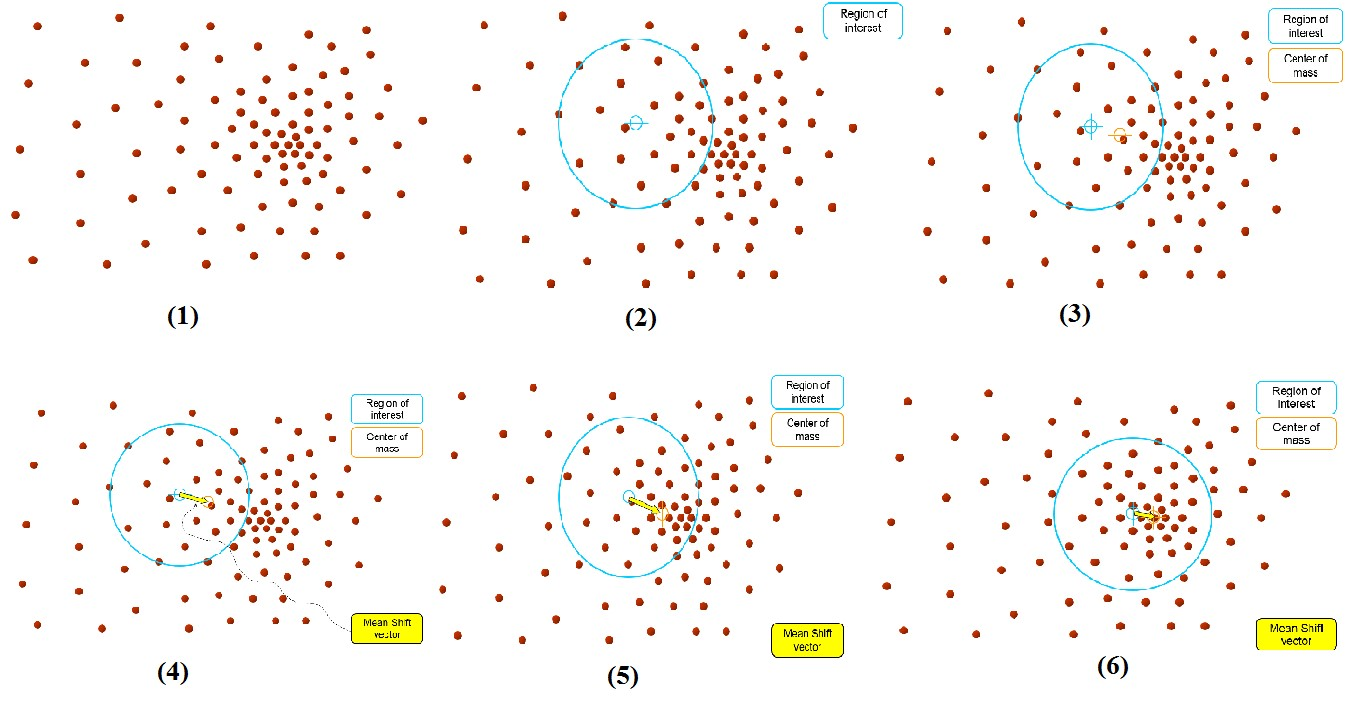
\includegraphics[width=12cm]{fig3.jpg}
\caption{ نحوه پیدا کردن محل با بیشترین تراکم به روش جابه‌جایی میانگین}
\label{pic-3}
\end{figure}



شکل \ref{pic-3} به رنگ زرد نشان داده‌شده است. بنابراین نقطه پیداشده در اولین تکرار این الگوریتم، همان نقطه زرد رنگ خواهد بود. بنابراین باید نقطه اولیه را به این نقطه انتقال دهیم. این کار توسط برداری انجام می‌شود که میانگین ناحیه را انتقال می‌دهد. بنابراین به این بردار، بردار جابه‌جایی میانگین (Mean Shift) گفته می‌شود. در بردار در شکل \ref{pic-4} نشان داده‌شده است. سپس نوبت اجرای همین مراحل برای همگرا شدن به متراکم‌ترین نقطه و مرکز جرم تابع است. بنابراین باید الگوریتم تکرار شود. تکرار‌های دوم و سوم الگوریتم در شکل‌های \ref{pic-5} و \ref{pic-6} نشان داده‌شده است.
بنابراین از این الگوریتم برای پیدا کردن نقطه‌ی ماکزیمم تابع و یا چگالی احتمال استفاده می‌شود. برای استفاده از این الگوریتم در ردیابی باید معیار شباهتی بین جسم مورد ردیابی و جسم موردنظر در فریم بعدی تعریف کنیم و سپس ماکزیمم این تابع شباهت را پیدا کنیم تا شبیه‌ترین جسم به جسم مورد ردیابی را در فریم بعدی پیدا کنیم. معیار‌هایی که به‌طور معمول تعریف می‌شوند شباهت هیستوگرام، بین جسم مورد ردیابی و جسم در فریم بعدی می‌باشند. یکی از این معیارها، فاصله باتاچریا  می‌باشد که بین دو تابع توزیع احتمال و یا هیستوگرام تعریف می‌شود.
در مقاله مورد بررسی، برای استفاده از الگوریتم جابه‌جایی میانگین به این شکل عمل می‌شود. ابتدا از جسم مورد ردیابی هیستوگرام رنگ گرفته می‌شود. برای تعریف هیستوگرام در این روش، یک تابع کرنل بر روی پنجره‌ای که در آن هیستوگرام می‌گیریم در نظر می‌گیریم. روند انجام این کار در شکل \ref{pic-4} نشان داده‌شده است. 
هسته نشان داده شده در این شکل گوسی می‌باشد که وزن بیشتری به پیکسل‌های مرکزی پنجره نسبت می‌دهد. همین‌طور یک نمونه هیستوگرام استخراج‌شده به این روش نیز در این شکل و در بخش (2) نشان داده‌شده است.
\begin{figure}[h]
\centering
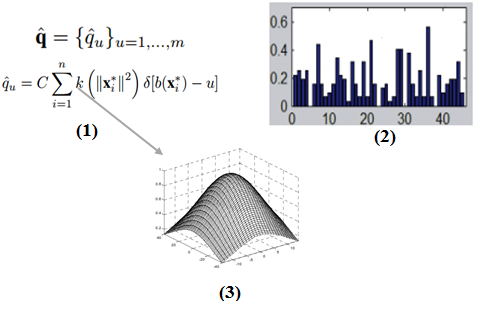
\includegraphics[scale=0.8]{fig4.png}
\caption{نحوه محاسبه هیستوگرام در روش جابه‌جایی میانگین}
\label{pic-4}
\end{figure}



سپس ناحیه‌ای در اطراف مکان قبلی جسم، در فریم کنونی برای جستجوی جسم در نظر گرفته می‌شود. در  این ناحیه از پنجره‌های هم‌اندازه با جسم اصلی هیستوگرام رنگ گرفته‌می‌شود. سپس مشابه‌ترین هیستوگرام به هیستوگرام جسم اصلی به‌عنوان مکان بعدی جسم در نظر گرفته می‌شود.
به همین شکل هیستوگرام ناحیه تست نیز استخراج می‌شود. سپس برای تعیین میزان شباهت این دو هیستوگرام ضریب Bhattacharya به‌صورت رابطه \ref{eq1} تعریف می‌شود.
\begin{equation}
\hat{\rho}(y)  \equiv \rho[\hat{p}(y),\hat{q}] = \sum_{u=1}^{m}{\sqrt{\hat{p}_u(y)\hat{q}_u}}
\label{eq1}
\end{equation}

در این رابطه، $\hat{p}(y)$ هیستوگرام ناحیه تست و $\hat{q}$ هیستوگرام اصلی جسم مورد ردیابی است. فاصله‌ی این دو هیستوگرام به‌صورت رابطه‌ی \ref{eq2} و با استفاده از ضریب باتاچریا $\hat{\rho}(y)$ تعریف می‌شود.
\begin{equation}
d(y) = \sqrt{1 - \hat{\rho}(y) }
\label{eq2}
\end{equation}

درواقع همان‌طور که پیش‌ازاین اشاره شد الگوریتم Mean-Shift برای تعیین ماکزیمم یک تابع مورد استفاده قرار می‌گیرد. در اینجا هم برای پیدا کردن ماکزیمم ضریب باتاچریا از الگوریتم Mean-Shift استفاده می‌کنیم. برای انجام این کار بعد از حل کردن روابط الگوریتم Mean-Shift و استفاده از ضریب باتاچریا به‌عنوان تابع موردنظر، به روابط   \ref{eq3} و \ref{eq4} می‌رسیم. 
\begin{equation}
\hat{y}=\frac{\sum_{i=1}^{nk}{x_iw_ig(\| \frac{\hat{y}_0-x_i}{h})\|}^2)}{\sum_{i=1}^{nk}{w_ig(\| \frac{\hat{y}_0-x_i}{h}\|^2)}}
\label{eq3}
\end{equation}

\begin{equation}
w_i=\sum_{u=1}^{m}{\sqrt{\frac{\hat{q}_u}{\hat{p}_u(\hat{y}_0)}}\delta[b(x_i)-u]}
\label{eq4}
\end{equation}
در این روابط $\hat{y}_0$ مکان قبلی جسم،  $\hat{y}$ مکان پیدا شده جسم توسط الگوریتم جابه‌جایی میانگین، $x$ مختصات پیکسل‌های تصویر، و $h$ پهنای باند کرنل مورد استفاده الگوریتم است که در این مقاله از کرنل گوسی استفاده شده است.
در هر بار اجرای الگوریتم مقدار ضریب باتاچریا افزایش می‌یابد و به نقطه‌ای با شباهت بیشتر دست پیدا می‌کنیم. این تکرار تا زمانی ادامه پیدا می‌کند که حد مطلوبی از دقت دست‌یافته باشیم. درواقع زمانی که مقدار جابه‌جایی حاصل از اجرای الگوریتم از حدی کوچک‌تر باشد، می‌توان اجرای الگوریتم را متوقف کرد.
در شکل \ref{pic-5} نتایج شبیه‌سازی ردیابی به این روش آورده شده است. همان‌طور که ملاحظه می‌شود این الگوریتم تا زمانی که ابعاد جسم موردنظر تغییر نکند، با دقت بالا قابلیت ردیابی جسم را دارد. اما زمانی که ابعاد جسم تغییر می‌کند، به دلیل اینکه ابعاد کرنل این الگوریتم ثابت است، در ردیابی جسم دچار مشکل می‌شود. از طرفی اگر بخواهیم در پارامترهای ردیابی، ابعاد کرنل را نیز تغییر بدهیم، پیچیدگی محاسباتی الگوریتم بسیار بالا می‌رود. زیرا باید جستجو را با ابعاد مختلف تکرار کنیم. به همین دلیل روش‌های زیادی برای مقابله با مشکل تغییر ابعاد جسم پیشنهاد شده است. در بخش بعدی روش مورد ارائه این مقاله برای تعیین ابعاد جدید جسم را بررسی می‌کنیم.

\begin{figure}[h]
\centering
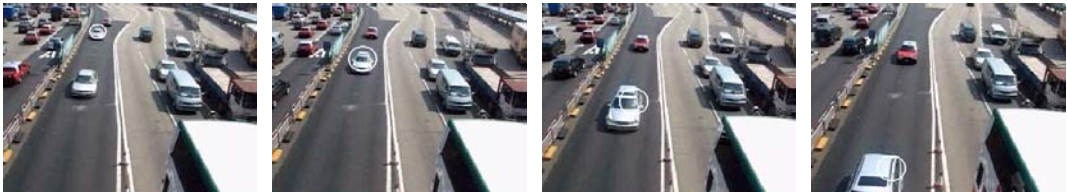
\includegraphics[width=12cm]{fig5.png}
\caption{شبیه‌سازی روش جابه‌جایی میانگین برای ردیابی اجسام با ابعاد ثابت}
\label{pic-5}
\end{figure}



\subsection{	محاسبه ابعاد جسم}
برای انجام این کار ابتدا همان‌طور که در شکل \ref{pic-2} مشاهده می‌شود، همان الگوریتم جابه‌جایی میانگین اجرا شده و شبیه‌ترین جسم به جسم اصلی و باهمان ابعاد قبلی به دست می‌آید. سپس از آنجایی که بین دو فریم متوالی ابعاد جسم تغییر ناگهانی ندارد، انتظار می‌رود بخش‌هایی از جسم اصلی در هر دو تصویر موجود باشد. با پیدا کردن نقاط متناظر بین این دو شکل، و محاسبه تغییر ابعاد آن‌ها می‌توان ابعاد جسم جدید را به دست آورد.
برای محاسبه ابعاد جسم جدید، ابتدا باید نقاط متناظر هر دو جسم را پیدا کنیم. برای اینکه بتوانیم این کار را با سرعت بالا انجام دهیم تا ردیابی هنوز قابلیت اجرا به‌صورت آنلاین را داشته باشد، از الگوریتم شناسایی گوشه‌های تصویر به روش
 FAST
 \cite{6Collins} 
 استفاده می‌کنیم. استفاده از این روش بهینگی زمانی الگوریتم را حفظ می‌کند. بعد از پیدا شدن این گوشه‌ها در هر دو تصویر، باید گوشه‌های متناظر باهم را شناسایی کنیم. برای انجام این کار از گوشه‌های یافت‌شده، الگوهایی استخراج‌شده و گوشه‌های پیداشده تصویر دوم مقایسه می‌شود و گوشه‌های متناظر پیدا می‌شوند.
این روش در شکل \ref{pic-6} نشان داده شده است. بعد از پیدا شدن گوشه‌ها، از آن‌ها الگوی HOG \footnote{Histograms of Gradient} استخراج می‌شود. این الگو با تقسیم کردن ناحیه‌ی اطراف گوشه، به 9 زیر بخش به دست می‌آید و هیستوگرام آن به دست می‌آید.

\begin{figure}[h]
\centering
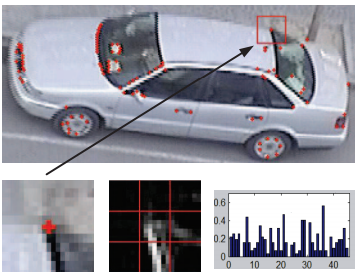
\includegraphics[scale=0.8]{fig6.png}
\caption{ روش ایجاد تناظر بین گوشه‌های پیدا شده در دو تصویر تست و اصلی}
\label{pic-6}
\end{figure}

بعد از اینکه گوشه‌های متناظر شناسایی شدند، زمان محاسبه ابعاد جسم جدید با توجه به دانستن ابعاد جسم در فریم قبلی است. برای انجام این کار از سه تبدیل مختلف استفاده کرده ایم affine استفاده می‌شود. از آنجایی که جسم می‌تواند دچار چرخش نیز شده‌باشد، این چرخش نیز در این رابطه 
زیر
      در نظر گرفته شده‌اند.
\\
\begin{center}
%\begin{equation}
\begin{minipage}{.5\linewidth}
\[
\begin{pmatrix}
{%
x_c \cr
y_c \cr
1
}
\end{pmatrix}
=
\begin{pmatrix}
{%
s_x \cos\theta & -s_x \sin\theta & t_x \cr
s_y \sin\theta & s_y \cos\theta & t_y \cr
0 & 0 & 1
}
\end{pmatrix}
\begin{pmatrix}
{%
x_p \cr
y_p \cr
1
}
\end{pmatrix}
\]
\end{minipage}\\
%\end{equation}
\label{mat1}
\end{center}
در این رابطه مختصات مربوط به فریم قبلی با اندیس p و فریم فعلی با اندیس c نامگذاری شده‌اند. با حل این دستگاه مختصات مقدار تغییر مقیاس در جهت x و y که به ترتیب با   و   و مقدار چرخش   مشخص می‌شود. این روند در شکل\ref{pic-7} نشان داده‌شده است.
\begin{figure}[h]
\centering
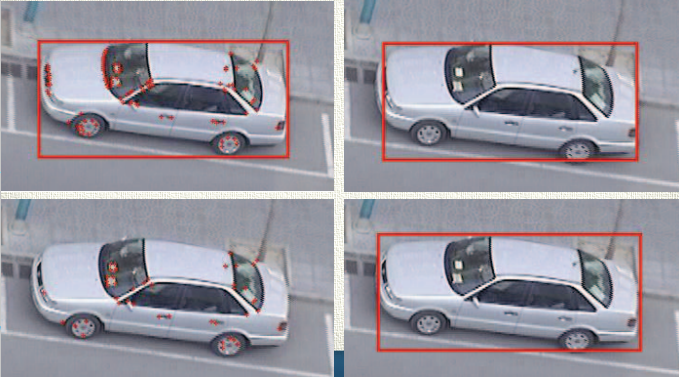
\includegraphics[width=12cm]{fig7.png}
\caption{نحوه محاسبه ابعاد پنجره هدف جدید}
\label{pic-7}
\end{figure}
حال که نحوه چگونگی محاسبه ابعاد جسم در فریم فعلی و نسبت تغییر پنجره هدف تعیین گردید، لازم می دانم به تین نکته اشاره داشته باشیم که یکی از مسائل مهم در این الگوریتم اعمال شده جهت تعیین ابعاد جسم در فریم جدید الگوریتم استخراج ویژگی و معیار تطبیق ویژگی ها است.
در الگوریتم بیان شده برای استخراج ویژگی از روش FAST corner و پارامتر محاسبه شده از آن HOG پیکسل هدف بود. اما برای تطبیق ویژگی های فریم قبلی و فریم کنونی از سه روش مجزا استفاده کرده ایم که ثابت شد که تفاوت نه چندان عمده اما قابل محسوسی در ویژگی های تطبیق داده شده می توان در آن ها یافت. این روش ها عبارتند از:
\begin{itemize}
\item	SE ، در روش اول با نام خطای مربع، ویژگی انتخاب شامل کمترین خطای مربع در بین زوج ویژگی های استخراج شده در فریم قبلی و فریم کنونی دارد به عبارنی برای ویژگی استخراج شده $g_j$ از فریم قبلی و ویژگی استخراج شده $h_i$ از فریم فعلی به دنبال $\forall i,j \in FAST_{feature} \min (h_i-g_j)^2 $ هستیم
\item	Kullback–Leibler ,براساس این معیار به دنبال $i$ و $j$ هستیم که مقدار زیر را بیشینه کند.

\begin{flushleft}
$D_{ij}=D_{jk}(H\|G)+D_{jk}(G\|H)=\sum_{i=1}^{l}{\ln\frac{H(i)+\epsilon}{G(i)+\epsilon}+\ln\frac{G(i)+\epsilon}{H(i)+\epsilon}}$
\end{flushleft}
\item	NSE ,براساس این معیار پس محاسبه خطای مربع مقادیر هیستوگرام ها حاصل بدست آمده را بر مجموع هستوگرام ها تقسیم می نماییم.
\end{itemize}
که این معیارها گاها جواب یکسان می دهند و گاهی جواب متفاوت. تجربه ثابت کرده معیار سوم یعنی $NSE$ بهترین معیار است. در شکل های \ref{pic-sim} \ref{pic-unsim} نمونه هایی از تشابه و اختلاف را برای معیار دوم و سوم مشاهده می نمایید.
\begin{figure}
\centering
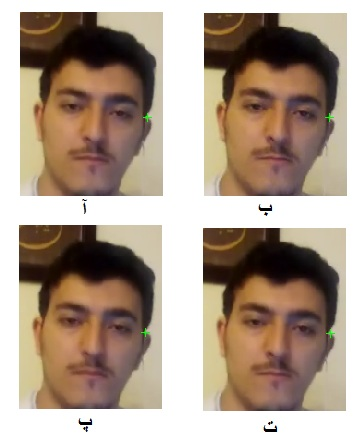
\includegraphics[width=12cm]{similar.jpg}
\caption{پاسخ دهی مشابه معیار Kullback و NSE در شکل آ و ب ویژگی های فریم قبل و فریم فعلی توسط NSE انتخاب شده است و در شکل پ و ت بهترین ویژگی ها توسط معیار Kullback انتخاب شده است}
\label{pic-sim}
\end{figure}

\begin{figure}
\centering
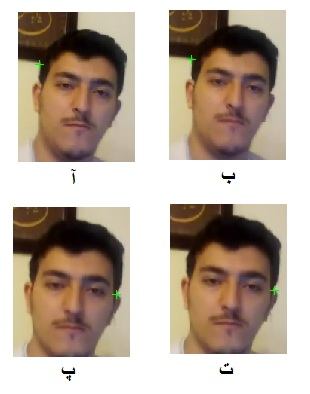
\includegraphics[width=12cm]{unsimilar.jpg}
\caption{پاسخ دهی متفاوت معیار Kullback و NSE در شکل آ و ب ویژگی های فریم قبل و فریم فعلی توسط NSE انتخاب شده است و در شکل پ و ت بهترین ویژگی ها توسط معیار Kullback انتخاب شده است}
\label{pic-unsim}
\end{figure}


\subsection{ به‌روزرسانی مدل جسم}
مدلی که از جسم برای ردیابی استخراج می‌شود، در این مقاله هیستوگرام رنگ می‌باشد. اما به دلیل تغییر شدت روشنایی و یا پوشیده شدن جسم مورد ردیابی، این مدل می‌تواند در طول ردیابی دچار تغییراتی بشود. بنابراین نیاز داریم که مدل جسم را با گذشت هر فریم به‌روزرسانی کنیم.
روشی که در این مقاله برای به‌روزرسانی هیستوگرام رنگ استخراج‌شده استفاده شده است، به این صورت است که هیستوگرام در هر فریم مطابق رابطه‌ی \ref{eq6} به‌روز می‌شود.
\begin{equation}
H_m=\alpha H_c + (1-\alpha)H_0
\label{eq6}
\end{equation}
که در آن $H_c$ هیستوگرام در فریم کنونی و      $H_0$	هیستوگرام اولیه استخراج‌شده از جسم اصلی می‌باشد. این دو هیستوگرام با ضریبی که بین [1و0] است باهم ادغام می‌شوند تا هیستوگرام به‌روز شود.

\subsection{ آزمایشات عملی}
برای مقایسه روش معرفی‌شده توسط این مقاله، نتایج شبیه‌سازی آن با روش‌های دیگری مقایسه شده است. این روش‌ها عبارتند از:
\begin{itemize}


\item	Adaptive MeanShift Tracker (AMST)
\item	MeanShift Blob Tracker (BT)
\item	Feature-Point Based Object Tracker (FPOT)
\end{itemize}

نتایج این مقایسه از نظر پیچیدگی محاسباتی و دقت ردیابی در جدول \ref{tab1} آورده‌شده است.
\begin{table}

\centering
\caption{ مقایسه روش مورد مطالعه مقاله با سایر روش‌ها از نظر پیچیدگی محاسباتی}

\label{tab1}

\begin{tabular}{|c|c|c|c|c|}

\hline
\cline{1-5} Trackers & AMST & BT& FPOT & Ours\\
\cline{1-5} Time per frame(ms) & 3.78 & 77.61 & 0.44 & 0.55 \\
\hline
\end{tabular}
\end{table}

\begin{table}
\centering
\label{tab2}
\begin{tabular}{|c|c|c|c|c|}

\hline
\cline{1-5} Image Seguences & AMST & BT& FPOT & Ours\\
\cline{1-5} Face & \underline{ 0.6807} & 0.6523 & 0.2023 & \textbf{ 0.7277} \\
\cline{1-5} SUV & \textbf{ 0.7942} & 0.5718 & 0.7013 & \underline{0.7754}\\
\cline{1-5} Walk & 0.6637 & 0.4014 & \underline{0.8317} & \textbf{0.8572} \\

\hline

\end{tabular}
\end{table}

همان‌طور که مشاهده می‌شود روش مقاله، در اغلب موارد بهترین دقت ردیابی را داشته است. همین‌طور از نظر پیچیدگی محاسباتی نیز با درنظرگرفتن دقت بالای آن، نتیجه خوبی داشته‌است. در شکل \ref{pic-7} و \ref{pic-8} نیز نتیجه شبیه‌سازی این روش روی ویدئویی که دارای تغییر ابعاد بسیار است، آورده‌شده است.
\begin{figure}
\centering
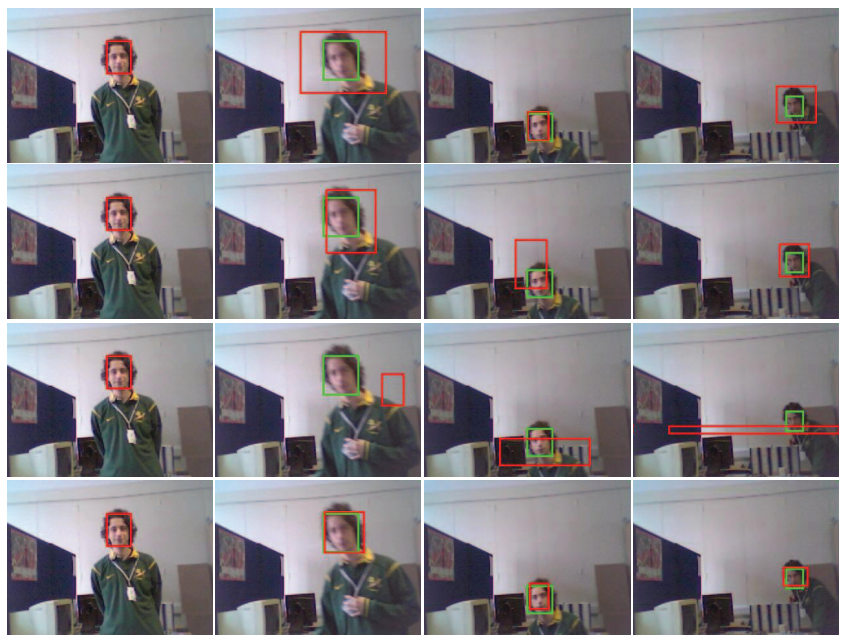
\includegraphics[width=12cm]{fig8.png}
\caption{نتیجه شبیه‌سازی روش مورد مطالعه مقاله بر روی ویدئو دارای تغییر ابعاد متوسط}
\label{pic-8}
\end{figure}

\begin{figure}
\centering
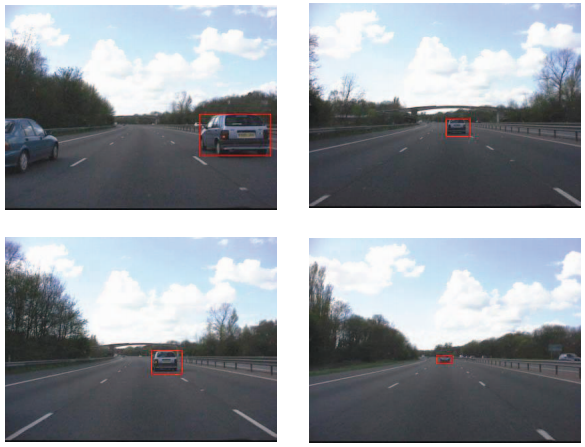
\includegraphics[scale=0.8]{fig9.png}
\caption{نتیجه شبیه‌سازی روش مورد مطالعه مقاله بر روی ویدئو دارای تغییر ابعاد زیاد}
\label{pic-9}
\end{figure}

 
\section{ پیشنهادات بهبود عملکرد روش ارائه‌شده}
در مساله ردیابی دستیابی به دقت ردیابی بالا و پیچیدگی محاسباتی پایین از اهمیت بسزایی برخوردار است. در این بخش دو پیشنهاد ارائه می‌شود که اولی برای افزایش دقت ردیابی، توام با کاهش پیچیدگی محاسباتی می‌باشد. پیشنهاد دوم هم استفاده از الگویی غیر از هیستوگرام رنگ می‌باشد که مقاومت ردیابی به تغییرات ظاهر را افزایش می‌دهد.

\subsection{ پیش‌بینی مکان جسم در فریم‌های بعدی با استفاده از فیلتر کالمن}
در این مقاله برای جستجوی جسم مورد ردیابی، در هر فریم، مستطیلی در اطراف مکان قبلی جسم درنظرگرفته می‌شود و در این مستطیل بزرگ، جسم موردنظر جستجو می‌شود. این کار باعث می‌شود در هر فریم مکان‌های زیادی برای پیدا کردن جسم جستجو شود و پیچیدگی محاسباتی افزایش چشمگیری پیدا می‌کند. برای رفع این مشکل استفاده از فیلتر کالمن برای پیش‌بینی مکان جسم در فریم‌های بعدی پیشنهاد می‌شود.
فیلتر کالمن روشی برای پیش‌بینی موقعیت جسم در فریم‌های بعدی، با توجه به مدل دینامیکی حرکت و مکان جسم در فریم‌های قبلی می‌باشد.
\cite{7Jiang}
 برای استفاده از این فیلتر باید ابتدا معادلات دینامیکی جسم را تعریف کرد. این معادلات لزومی ندارد که به‌طور دقیق در مورد جسم صادق باشد، زیرا با پیدا شدن مکان دقیق جسم در هر فریم، فیلتر کالمن این توانایی را دارد که معادلات حرکت را اصلاح و خطا را کاهش دهد.
بنابراین می‌توان با استفاده از مکان جسم در فریم‌های قبلی و با توجه به معادلات دینامیکی حرکت جسم (مثلاً حرکت با شتاب ثابت) ، مکان متحرک را در فریم بعدی پیش‌بینی کرد و در اطراف این پیش‌بینی به دنبال جسم گشت. درواقع این کار هزینه محاسباتی را بسیار پایین می‌آورد.زیرا دامنه جستجو را تا حد زیادی محدود می‌کند.

\subsection{ استفاده از الگوهای بافت تصویر به جای هیستوگرام رنگ}
الگویی که در این مقاله از آن استفاده‌شده است، هیستوگرام رنگ می‌باشد. اما استفاده از هیستوگرام رنگ، در ردیابی می‌تواند مشکلات زیادی را ایجاد کند. از جمله اینکه ظاهر جسم به دلیل تغییرات روشنایی می‌تواند تا حدی تغییر کند که دیگر رنگی مشابه فریم‌های قبلی نداشته باشد. همین‌طور این موضوع می‌تواند باعث ایجاد مشکلاتی در ردیابی اجسام همرنگ شود.
به جای استفاده از این کار می‌توان از توصیف کننده‌های بافت مانند LBP و یا
 LPQ
  \cite{8Ning}
  استفاده کرد که به این موارد مقاوم هستند و دقت ردیابی را افزایش می‌دهند.

\begin{thebibliography}{9}

\begin{LTRitems}
\resetlatinfont

\bibitem{1Bedfold}
B. Benfold and I. Reid, “Stable multi-target tracking in real-time surveillance video,” in IEEE Conference on Computer Vision and Pattern Recognition, 2011, pp. 3457–3464.

\bibitem{2SVT}
S. Avidan, “Support vector tracking,” IEEE Transactions on Pattern Analysis and Machine Intelligence, vol. 26, no. 8, pp. 1064–1072, 2004.

\bibitem{3Oikonomidis}
I. Oikonomidis, N. Kyriazis, and A. A. Argyros, “Tracking the articulated motion of two strongly interacting hands,” in IEEE Conference on Computer Vision and Pattern Recognition, 2012, pp. 1862–1869.

\bibitem{4Zhang}
Z. Zhang, R. Sa, and Y. Wang, “A real time object tracking approach for mobile robot visual servo control,” in 2011 First Asian Conference on Pattern Recognition (ACPR), 2011, pp. 500–504.

\bibitem{5Comaniciu}
D. Comaniciu, V. Ramesh, and P. Meer, “Kernel-based object tracking,” IEEE Transactions on Pattern Analysis and Machine Intelligence, vol. 25, no. 5, pp. 564–577, 2003.

\bibitem{6Collins}
R. T. Collins, “Mean-shift blob tracking through scale space,” in IEEE Computer Society Conference on CVPR, 2003., vol. 2, 2003, pp. II:234–240.
\bibitem{7Jiang}
Z.-L. Jiang, S.-F. Li, and D.-F. Gao, “An adaptive mean shift tracking method using multiscale images,” in International Conference on Wavelet Analysis and Pattern Recognition, vol. 3, 2007, pp. 1060–1066.

\bibitem{8Ning}
J. Ning, L. Zhang, D. Zhang, and C. Wu, “Scale and orientation adaptive mean shift tracking,” Computer Vision, IET, vol. 6, no. 1, pp. 52–61, 2012.

\bibitem{9Vojir}
T. Vojir, J. Noskova, and J. Matas, “Robust scale-adaptive mean-shift for tracking,” in Image Analysis. Springer, 2013, pp. 652–663.

\bibitem{10Shi}
J. Shi and C. Tomasi, “Good features to track,” in IEEE Computer Society Conference on CVPR., 1994, pp. 593–600.

\bibitem{11Zhou}
H. Zhou, Y. Yuan, and C. Shi, “Object tracking using SIFT features and mean shift,” Computer Vision and Image Understanding, vol. 113,no. 3, pp. 345–352, 2009.

\bibitem{12Rublee}
E. Rublee, V. Rabaud, K. Konolige, and G. Bradski, “ORB: An efficient alternative to SIFT or SURF,” in IEEE International Conference on Computer Vision, 2011, pp. 2564–2571.

\bibitem{13Rosten}
E. Rosten, R. Porter, and T. Drummond, “Faster and better: A machine learning approach to corner detection,” IEEE Trans. on Pattern Analysis and Machine Intelligence, vol. 32, no. 1, pp. 105–119, 2010.

\bibitem{14Dalal}
N. Dalal and B. Triggs, “Histograms of oriented gradients for human detection,” in IEEE Computer Society Conference on CVPR, 2005.,vol. 1, 2005, pp. 886–893.

\bibitem{15Wang}
Y. Wang, Y. Tan, and J. Tian, “New tracking algorithm based on mean shift with adaptive bandwidth of kernel function,” Journal of Data Acquisition and Processing, pp. 762–766, 2009.

\bibitem{16Comaniciu}
D. Comaniciu and P. Meer, “Mean shift: A robust approach toward feature space analysis,” IEEE Transactions on Pattern Analysis and Machine Intelligence, vol. 24, no. 5, pp. 603–619, 2002.

\bibitem{17Wu}
G. Wu, Y. Xu, X. Yang, Q. Yan, and K. Gu, “Robust object tracking with bidirectional corner matching and trajectory smoothness algorithm,” in 2012 IEEE 14th International Workshop on Multimedia Signal Processing (MMSP), 2012, pp. 294–298.

\bibitem{18Leichter}
I. Leichter, M. Lindenbaum, and E. Rivlin, “Tracking by affine kernel
transformations using color and boundary cues,” IEEE Transactions on
Pattern Analysis and Machine Intelligence, vol. 31, no. 1, pp. 164–171,
2009.

\bibitem{19Kim}
D.-H. Kim, H.-K. Kim, S.-J. Ko et al., “Spatial color histogram based
center voting method for subsequent object tracking and segmentation,”
Image and Vision Computing, vol. 29, no. 12, pp. 850–860, 2011.

\bibitem{20SPEVI}
SPEVI dataset, “http://www.eecs.qmul.ac.uk/andrea/spevi .html.” ˜

\bibitem{21PET2001}
PETS2001, “http://www.cvg.rdg.ac.uk/pets2001,” 2001.

\bibitem{22CAVIAR}
CAVIAR Test Case Scenarios, “http://groups.inf.ed.ac.uk/vision/caviar/caviardata1,” 2004.

\bibitem{}



\end{LTRitems}
\end{thebibliography}


\end{document}
